\documentclass[11pt]{article}
\usepackage{amsmath,amssymb,amsthm}
\usepackage[pdftex]{graphicx}
\usepackage{fancyhdr}
\pagestyle{fancy}

\setlength{\headheight}{0.75in}
\setlength{\oddsidemargin}{0in}
\setlength{\evensidemargin}{0in}
\setlength{\voffset}{-1.0in}
\setlength{\headsep}{10pt}
\setlength{\textwidth}{6.5in}
\setlength{\headwidth}{6.5in}
\setlength{\textheight}{8.5in}

\lhead{}
\chead{Lending Club Project Report}
\rhead{Jim Tao}
\lfoot{}
\cfoot{}
\rfoot{\thepage}
\renewcommand{\headrulewidth}{0.5pt}
\renewcommand{\footrulewidth}{0.3pt}
\setlength{\textwidth}{6.5in}

\begin{document}
\begin{flushleft}
{\em What characteristics make a loan most likely to be fully paid?
What characteristics make a loan most likely to be charged off?
To what extent can we train machine learning models to predict whether a	loan will be fully paid or charged off?}
\end{flushleft}

Data wrangling shows us that the target feature to predict is loan status
(fully paid or charged off). After transforming these categorical features
into numerical features, we apply and compare four machine learning techniques.
We find that logistic regression has 63\% balanced accuracy (average recall for
each class) and has the best explanatory power, although random forest and
XGBoost are also informative and perform almost as well with 61\% and 62\%
balanced accuracy, respectively.

Using logistic regression, we are able to determine the four traits most
strongly associated with loans that are fully paid. They are, in order of
importance, mean FICO score, annual income, credit card related purpose,
and debt consolidation related purpose, with logistic regression coefficients
$0.38$, $0.29$, $0.18$, and $0.13$, respectively.
We are also able to determine the four traits most strongly
associated with loans that get charged off. They are, in order of importance,
longer term loans (60 months instead of 36 months), inquiries within the last
six months, credit utilization rate, and small business related purpose,
with logistic regression coefficients $-0.38$, $-0.23$, $-0.16$, and $-0.15$
respectively.

According to random forest classification, monthly debt to income and total
credit balance are also important and in the top four important features:
\begin{center}
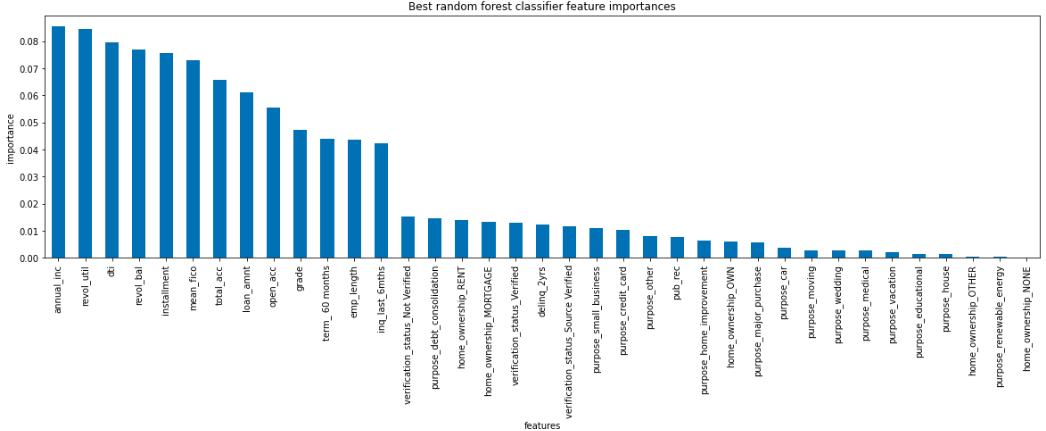
\includegraphics[scale=0.35]{random-forest-feature-importances.png}
\end{center}
According to XGBoost classification, loan grade is also important and in the
top four important features:
\begin{center}
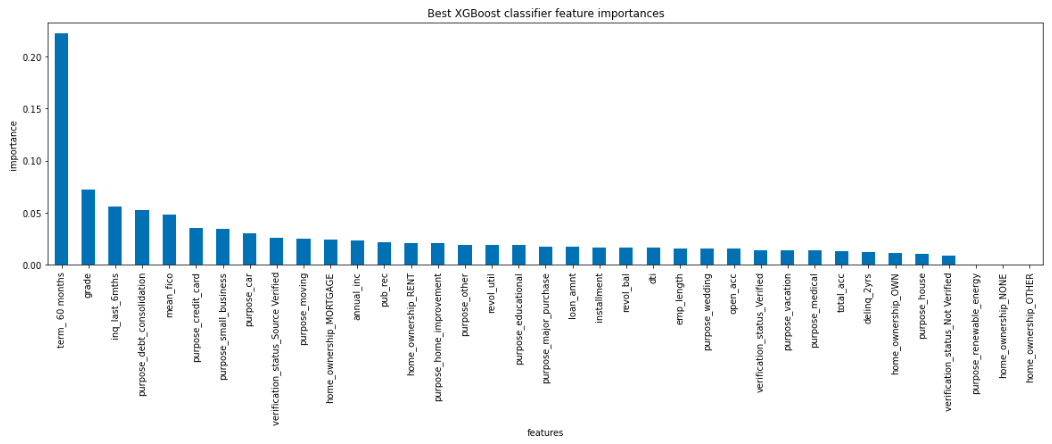
\includegraphics[scale=0.35]{xgboost-feature-importances.png}
\end{center}
\end{document}
